\section{Clasificación de arquitecturas paralelas}\label{clasificacion-arq-paralelas}

\subsection{Computación paralela y computación distribuida}\label{computacion-par-distribuida}

La \textbf{computación paralela} estudia los aspectos hardware y sofrware relacionados con el desarrollo y ejecución de aplicaciones en un sistema de cómputo compuesto por múltiples núcleos, procesadores o computadores que es visto externamente como una unidad autónoma.
Por otro lado, la \textbf{computación distribuida} estudia los aspectos hardware y software relacionados con el desarrollo y ejecución de aplicaciones en un sistema distribuido, que es una colección de recursos autónomos situados en distintas localizaciones físicas.
En general, nos referimos a computación paralela cuando el trabajo es realizado por un único computador y a computación distribuida cuando es realizado por varios.

\subsubsection{Computación grid y \textit{cloud}}

La \textbf{computación distribuida a baja escala} estudia los aspectos relacionados con el desarrollo y ejecución de aplicaciones en un conjunto de computadores de un único dominio situados en distintas localizaciones físicas conectadas a través de una infraestructura de red local
Por su parte, la \textbf{computación grid} estudia los aspectos relacionados con el desarrolo y ejecución de aplicaciones en un conjunto de computadores de varios dominios geográficamente distribuidos conectados con una infraestructura de telecomunicaciones.

La computación \textbf{\textit{cloud}} estudia los aspectos relacionados con el desarrollo y ejecución de aplicaciones en un sistema \textit{cloud}, que es un sistema que ofrece servicios de infraestructura, plataforma y/o software a los que se accede normalmente mediante una interfaz de auto-servicio.
Estos servicios son de pago (\textit{pay-per-use}) y ofrece recursos virtuales que, al ser una abstracción de los físicos, parecen ilimitados en número y capacidad y son gestionados de forma inmediata sin interacción con el proveedor.
Estos recursos soportan el acceso de múltiples clientes y están conectdos con métodos estándar independientes de la plataforma de acceso.

\subsection{Clasificaciones de arquitecturas y sistemas paralelos}\label{clasificaciones-arq-sistemas-paralelos}

\subsubsection{Clasificación comercial: Segmento de mercado}

En función del consumidor objetivo de los computadores podemos clasificarlos de mayor a menor precio y prestaciones:

\begin{center}
\begin{tabular}{l r r}
\textbf{Computador}       & \textbf{Núcleos} & \textbf{Precio (€)} \\
\toprule
Supercomputadores         & $128<x$          & $5000000<x$         \\
Servidores de gama alta   & $4<x<256$        & $750000<x<10000000$ \\
Servidores de gama media  & $2<x<64$         & $50000<x<1000000$   \\
Servidores de gama baja   & $2<x<16$         & $1000<x<10000$      \\
PCs y WorkStations        & $x<4$            & $x<10000$           \\
Computadores empotrados   & $---$            & $---$               \\
\end{tabular}
\end{center}

Los computadores externos (de escritorio, portátiles, servidores, clústers\ldots) se utilizan para todo tipo de aplicaciones, ya sean de oficina, entretenimiento, procesamiento de trasacciones (OLTP), sistemas de soporte de decisiones (DSS), científicas, animación\ldots
Por su parte, los computadores empotrados se utilizan para aplicaciones de propósito específico, como videojuegos, coches, teléfonos, electrodomésticos\ldots
Estos últimos tienen restricciones como un consumo de potencia, precio y tamaño reducidos y que deben realizar cómputos en tiempo real.

\subsubsection{Clasificación de Flynn de arquitecturas}

En 1972, Michael J. Flynn propone el siguiente esquema de clasificación de arquitecturas en función del flujo de instrucciones y datos:

\begin{figure}
\begin{center}
\begin{tabular}{C{6.5cm} | C{6.5cm}}
\textbf{SISD}                              & \textbf{MISD}                                    \\
\textit{Single Instruction, Single Data}   & \textit{Multiple Instruction, Single Data}       \\
Un núcleo procesador                       &                                                  \\
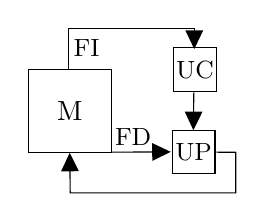
\begin{tikzpicture}[x=0.75pt,y=0.75pt,yscale=-1,xscale=1]
%uncomment if require: \path (0,235); %set diagram left start at 0, and has height of 235

%Shape: Rectangle [id:dp7536045366950691]
\draw   (90.33,80.33) -- (130.33,80.33) -- (130.33,120.33) -- (90.33,120.33) -- cycle ;
%Shape: Rectangle [id:dp09644128938666119]
\draw   (160.33,70) -- (181,70) -- (181,91) -- (160.33,91) -- cycle ;
%Shape: Rectangle [id:dp2241873458228455]
\draw   (159.67,109.67) -- (180.33,109.67) -- (180.33,130.67) -- (159.67,130.67) -- cycle ;
%Straight Lines [id:da17387488972120801]
\draw    (181,120.33) -- (190.33,120.39) -- (190.33,139.94) -- (110.56,139.94) -- (110.37,123.61) ;
\draw [shift={(110.33,120.61)}, rotate = 449.34] [fill={rgb, 255:red, 0; green, 0; blue, 0 }  ][line width=0.08]  [draw opacity=0] (8.93,-4.29) -- (0,0) -- (8.93,4.29) -- cycle    ;
%Straight Lines [id:da8399493952704167]
\draw    (130.33,120.33) -- (156,120.18) ;
\draw [shift={(159,120.17)}, rotate = 539.6700000000001] [fill={rgb, 255:red, 0; green, 0; blue, 0 }  ][line width=0.08]  [draw opacity=0] (8.93,-4.29) -- (0,0) -- (8.93,4.29) -- cycle    ;
%Straight Lines [id:da49329600167598175]
\draw    (170.11,91.5) -- (169.93,106.72) ;
\draw [shift={(169.89,109.72)}, rotate = 270.7] [fill={rgb, 255:red, 0; green, 0; blue, 0 }  ][line width=0.08]  [draw opacity=0] (8.93,-4.29) -- (0,0) -- (8.93,4.29) -- cycle    ;
%Straight Lines [id:da8478353646832082]
\draw    (109.89,80.17) -- (109.89,60.61) -- (170.33,60.61) -- (170.33,67.61) ;
\draw [shift={(170.33,70.61)}, rotate = 270] [fill={rgb, 255:red, 0; green, 0; blue, 0 }  ][line width=0.08]  [draw opacity=0] (8.93,-4.29) -- (0,0) -- (8.93,4.29) -- cycle    ;

% Text Node
\draw (110.33,100.67) node   [align=left] {M};
% Text Node
\draw (170.67,80.5) node   [align=left] {{\small UC}};
% Text Node
\draw (170,120.17) node   [align=left] {{\small UP}};
% Text Node
\draw (140.89,112.89) node   [align=left] {{\small FD}};
% Text Node
\draw (118.44,70) node   [align=left] {{\small FI}};
\end{tikzpicture}
                     & 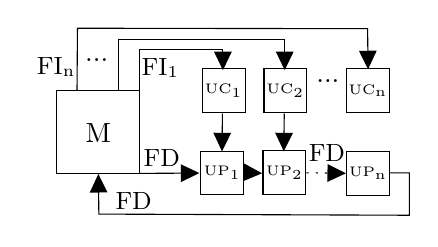
\begin{tikzpicture}[x=0.75pt,y=0.75pt,yscale=-1,xscale=1]
%uncomment if require: \path (0,235); %set diagram left start at 0, and has height of 235

%Shape: Rectangle [id:dp7536045366950691]
\draw   (90.33,80.33) -- (130.33,80.33) -- (130.33,120.33) -- (90.33,120.33) -- cycle ;
%Shape: Rectangle [id:dp09644128938666119]
\draw   (160.33,70) -- (181,70) -- (181,91) -- (160.33,91) -- cycle ;
%Shape: Rectangle [id:dp2241873458228455]
\draw   (159.67,109.67) -- (180.33,109.67) -- (180.33,130.67) -- (159.67,130.67) -- cycle ;
%Straight Lines [id:da17387488972120801]
\draw    (250.4,120.05) -- (260.18,120.05) -- (260.18,140.49) -- (110.56,139.94) -- (110.37,123.61) ;
\draw [shift={(110.33,120.61)}, rotate = 449.34] [fill={rgb, 255:red, 0; green, 0; blue, 0 }  ][line width=0.08]  [draw opacity=0] (8.93,-4.29) -- (0,0) -- (8.93,4.29) -- cycle    ;
%Straight Lines [id:da8399493952704167]
\draw    (130.33,120.33) -- (156,120.18) ;
\draw [shift={(159,120.17)}, rotate = 539.6700000000001] [fill={rgb, 255:red, 0; green, 0; blue, 0 }  ][line width=0.08]  [draw opacity=0] (8.93,-4.29) -- (0,0) -- (8.93,4.29) -- cycle    ;
%Straight Lines [id:da49329600167598175]
\draw    (170.11,91.5) -- (169.93,106.72) ;
\draw [shift={(169.89,109.72)}, rotate = 270.7] [fill={rgb, 255:red, 0; green, 0; blue, 0 }  ][line width=0.08]  [draw opacity=0] (8.93,-4.29) -- (0,0) -- (8.93,4.29) -- cycle    ;
%Straight Lines [id:da8478353646832082]
\draw    (130.33,80.33) -- (130.33,60.61) -- (170.33,60.61) -- (170.33,67.61) ;
\draw [shift={(170.33,70.61)}, rotate = 270] [fill={rgb, 255:red, 0; green, 0; blue, 0 }  ][line width=0.08]  [draw opacity=0] (8.93,-4.29) -- (0,0) -- (8.93,4.29) -- cycle    ;
%Shape: Rectangle [id:dp901514594846435]
\draw   (190.11,70) -- (210.78,70) -- (210.78,91) -- (190.11,91) -- cycle ;
%Straight Lines [id:da27835153565454673]
\draw    (199.89,91.5) -- (199.7,106.72) ;
\draw [shift={(199.67,109.72)}, rotate = 270.7] [fill={rgb, 255:red, 0; green, 0; blue, 0 }  ][line width=0.08]  [draw opacity=0] (8.93,-4.29) -- (0,0) -- (8.93,4.29) -- cycle    ;
%Straight Lines [id:da807958048653149]
\draw    (119.89,80.83) -- (119.89,55.94) -- (200.11,55.94) -- (200.11,67.61) ;
\draw [shift={(200.11,70.61)}, rotate = 270] [fill={rgb, 255:red, 0; green, 0; blue, 0 }  ][line width=0.08]  [draw opacity=0] (8.93,-4.29) -- (0,0) -- (8.93,4.29) -- cycle    ;
%Shape: Rectangle [id:dp6400885094204286]
\draw   (189.67,109.44) -- (210.33,109.44) -- (210.33,130.44) -- (189.67,130.44) -- cycle ;
%Straight Lines [id:da8803237857270745]
\draw    (180.54,119.83) -- (186.21,120.12) ;
\draw [shift={(189.2,120.27)}, rotate = 182.94] [fill={rgb, 255:red, 0; green, 0; blue, 0 }  ][line width=0.08]  [draw opacity=0] (8.93,-4.29) -- (0,0) -- (8.93,4.29) -- cycle    ;
%Straight Lines [id:da16287790070948704]
\draw  [dash pattern={on 0.84pt off 2.51pt}]  (210.51,120.05) -- (226.63,120.24) ;
\draw [shift={(229.63,120.27)}, rotate = 180.67] [fill={rgb, 255:red, 0; green, 0; blue, 0 }  ][line width=0.08]  [draw opacity=0] (8.93,-4.29) -- (0,0) -- (8.93,4.29) -- cycle    ;
%Shape: Rectangle [id:dp22681131917528252]
\draw   (229.89,70) -- (250.56,70) -- (250.56,91) -- (229.89,91) -- cycle ;
%Shape: Rectangle [id:dp6689432855617605]
\draw   (229.89,109.78) -- (250.56,109.78) -- (250.56,130.78) -- (229.89,130.78) -- cycle ;
%Straight Lines [id:da6654571954481253]
\draw    (100.04,80.17) -- (100.26,50.39) -- (240.04,50.61) -- (240.23,67.17) ;
\draw [shift={(240.26,70.17)}, rotate = 269.35] [fill={rgb, 255:red, 0; green, 0; blue, 0 }  ][line width=0.08]  [draw opacity=0] (8.93,-4.29) -- (0,0) -- (8.93,4.29) -- cycle    ;

% Text Node
\draw (110.33,100.67) node   [align=left] {M};
% Text Node
\draw (170.67,80.5) node   [align=left] {{\tiny UC\textsubscript{1}}};
% Text Node
\draw (170,120.17) node   [align=left] {{\tiny UP\textsubscript{1}}};
% Text Node
\draw (140.89,112.89) node   [align=left] {{\small FD}};
% Text Node
\draw (140.22,69.56) node   [align=left] {{\small FI\textsubscript{1}}};
% Text Node
\draw (200.44,80.5) node   [align=left] {{\tiny UC\textsubscript{2}}};
% Text Node
\draw (220.89,75.67) node   [align=left] {...};
% Text Node
\draw (109.56,65.67) node   [align=left] {...};
% Text Node
\draw (200,119.94) node   [align=left] {{\tiny UP\textsubscript{2}}};
% Text Node
\draw (240.22,80.5) node   [align=left] {{\tiny UC\textsubscript{n}}};
% Text Node
\draw (240.22,120.28) node   [align=left] {{\tiny UP\textsubscript{n}}};
% Text Node
\draw (220.44,110.44) node   [align=left] {{\small FD}};
% Text Node
\draw (127.33,133.56) node   [align=left] {{\small FD}};
% Text Node
\draw (90,69.11) node   [align=left] {{\small FI\textsubscript{n}}};
\end{tikzpicture}
                           \\
\hline
\textbf{SIMD}                              & \textbf{MIMD}                                    \\
\textit{Single Instruction, Multiple Data} & \textit{Multiple Instruction, Multiple Data}     \\
GPU, procesadores matriciales              & Multicores, multiprocesadores, multicomputadores \\
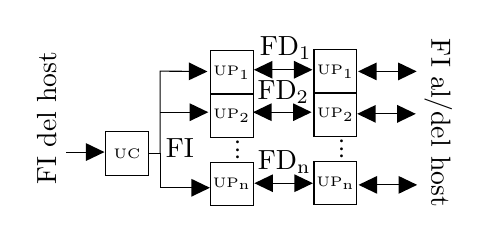
\begin{tikzpicture}[x=0.75pt,y=0.75pt,yscale=-1,xscale=1]
%uncomment if require: \path (0,235); %set diagram left start at 0, and has height of 235

%Shape: Rectangle [id:dp09644128938666119]
\draw   (49.47,89.78) -- (70.13,89.78) -- (70.13,110.78) -- (49.47,110.78) -- cycle ;
%Shape: Rectangle [id:dp2241873458228455]
\draw   (99.89,50.78) -- (120.56,50.78) -- (120.56,71.78) -- (99.89,71.78) -- cycle ;
%Shape: Rectangle [id:dp6400885094204286]
\draw   (99.89,71.44) -- (120.56,71.44) -- (120.56,92.44) -- (99.89,92.44) -- cycle ;
%Straight Lines [id:da8803237857270745]
\draw    (123.93,59.94) -- (146.15,59.94) ;
\draw [shift={(149.15,59.94)}, rotate = 180] [fill={rgb, 255:red, 0; green, 0; blue, 0 }  ][line width=0.08]  [draw opacity=0] (8.93,-4.29) -- (0,0) -- (8.93,4.29) -- cycle    ;
\draw [shift={(120.93,59.94)}, rotate = 0] [fill={rgb, 255:red, 0; green, 0; blue, 0 }  ][line width=0.08]  [draw opacity=0] (8.93,-4.29) -- (0,0) -- (8.93,4.29) -- cycle    ;
%Shape: Rectangle [id:dp6689432855617605]
\draw   (99.89,104.44) -- (120.56,104.44) -- (120.56,125.44) -- (99.89,125.44) -- cycle ;
%Shape: Rectangle [id:dp12722852093695813]
\draw   (149.89,50.33) -- (170.56,50.33) -- (170.56,71.33) -- (149.89,71.33) -- cycle ;
%Shape: Rectangle [id:dp3209291793254261]
\draw   (149.89,71) -- (170.56,71) -- (170.56,92) -- (149.89,92) -- cycle ;
%Shape: Rectangle [id:dp37749433061535154]
\draw   (149.89,104) -- (170.56,104) -- (170.56,125) -- (149.89,125) -- cycle ;
%Straight Lines [id:da6732803039595562]
\draw    (123.49,80.39) -- (145.71,80.39) ;
\draw [shift={(148.71,80.39)}, rotate = 180] [fill={rgb, 255:red, 0; green, 0; blue, 0 }  ][line width=0.08]  [draw opacity=0] (8.93,-4.29) -- (0,0) -- (8.93,4.29) -- cycle    ;
\draw [shift={(120.49,80.39)}, rotate = 0] [fill={rgb, 255:red, 0; green, 0; blue, 0 }  ][line width=0.08]  [draw opacity=0] (8.93,-4.29) -- (0,0) -- (8.93,4.29) -- cycle    ;
%Straight Lines [id:da14623578433410467]
\draw    (124.15,114.61) -- (146.37,114.61) ;
\draw [shift={(149.37,114.61)}, rotate = 180] [fill={rgb, 255:red, 0; green, 0; blue, 0 }  ][line width=0.08]  [draw opacity=0] (8.93,-4.29) -- (0,0) -- (8.93,4.29) -- cycle    ;
\draw [shift={(121.15,114.61)}, rotate = 0] [fill={rgb, 255:red, 0; green, 0; blue, 0 }  ][line width=0.08]  [draw opacity=0] (8.93,-4.29) -- (0,0) -- (8.93,4.29) -- cycle    ;
%Straight Lines [id:da5295276643399028]
\draw    (70.34,100.2) -- (75.74,100.2) -- (75.74,116.8) -- (96.74,116.8) ;
\draw [shift={(99.74,116.8)}, rotate = 180] [fill={rgb, 255:red, 0; green, 0; blue, 0 }  ][line width=0.08]  [draw opacity=0] (8.93,-4.29) -- (0,0) -- (8.93,4.29) -- cycle    ;
%Straight Lines [id:da5426076285509875]
\draw    (75.74,100.2) -- (75.74,60.6) -- (95.54,60.77) ;
\draw [shift={(98.54,60.8)}, rotate = 180.5] [fill={rgb, 255:red, 0; green, 0; blue, 0 }  ][line width=0.08]  [draw opacity=0] (8.93,-4.29) -- (0,0) -- (8.93,4.29) -- cycle    ;
%Straight Lines [id:da21553682836254784]
\draw    (75.74,80.4) -- (95.94,80.4) ;
\draw [shift={(98.94,80.4)}, rotate = 180] [fill={rgb, 255:red, 0; green, 0; blue, 0 }  ][line width=0.08]  [draw opacity=0] (8.93,-4.29) -- (0,0) -- (8.93,4.29) -- cycle    ;
%Straight Lines [id:da07605893617389348]
\draw    (174.13,60.74) -- (196.35,60.74) ;
\draw [shift={(199.35,60.74)}, rotate = 180] [fill={rgb, 255:red, 0; green, 0; blue, 0 }  ][line width=0.08]  [draw opacity=0] (8.93,-4.29) -- (0,0) -- (8.93,4.29) -- cycle    ;
\draw [shift={(171.13,60.74)}, rotate = 0] [fill={rgb, 255:red, 0; green, 0; blue, 0 }  ][line width=0.08]  [draw opacity=0] (8.93,-4.29) -- (0,0) -- (8.93,4.29) -- cycle    ;
%Straight Lines [id:da10873674757976892]
\draw    (173.69,81.19) -- (195.91,81.19) ;
\draw [shift={(198.91,81.19)}, rotate = 180] [fill={rgb, 255:red, 0; green, 0; blue, 0 }  ][line width=0.08]  [draw opacity=0] (8.93,-4.29) -- (0,0) -- (8.93,4.29) -- cycle    ;
\draw [shift={(170.69,81.19)}, rotate = 0] [fill={rgb, 255:red, 0; green, 0; blue, 0 }  ][line width=0.08]  [draw opacity=0] (8.93,-4.29) -- (0,0) -- (8.93,4.29) -- cycle    ;
%Straight Lines [id:da1846794210706837]
\draw    (174.35,115.41) -- (196.57,115.41) ;
\draw [shift={(199.57,115.41)}, rotate = 180] [fill={rgb, 255:red, 0; green, 0; blue, 0 }  ][line width=0.08]  [draw opacity=0] (8.93,-4.29) -- (0,0) -- (8.93,4.29) -- cycle    ;
\draw [shift={(171.35,115.41)}, rotate = 0] [fill={rgb, 255:red, 0; green, 0; blue, 0 }  ][line width=0.08]  [draw opacity=0] (8.93,-4.29) -- (0,0) -- (8.93,4.29) -- cycle    ;
%Straight Lines [id:da11974971166580506]
\draw    (30.54,99.6) -- (45.94,99.6) ;
\draw [shift={(48.94,99.6)}, rotate = 180] [fill={rgb, 255:red, 0; green, 0; blue, 0 }  ][line width=0.08]  [draw opacity=0] (8.93,-4.29) -- (0,0) -- (8.93,4.29) -- cycle    ;

% Text Node
\draw (59.8,100.28) node   [align=left] {{\tiny UC}};
% Text Node
\draw (110.22,61.28) node   [align=left] {{\tiny UP\textsubscript{1}}};
% Text Node
\draw (110.22,81.94) node   [align=left] {{\tiny UP\textsubscript{2}}};
% Text Node
\draw (110.22,114.94) node   [align=left] {{\tiny UP\textsubscript{n}}};
% Text Node
\draw (113.11,98.56) node  [rotate=-90] [align=left] {...};
% Text Node
\draw (160.22,60.83) node   [align=left] {{\tiny UP\textsubscript{1}}};
% Text Node
\draw (160.22,81.5) node   [align=left] {{\tiny UP\textsubscript{2}}};
% Text Node
\draw (160.22,114.5) node   [align=left] {{\tiny UP\textsubscript{n}}};
% Text Node
\draw (163.11,98.11) node  [rotate=-90] [align=left] {...};
% Text Node
\draw (136.22,49.67) node   [align=left] {FD\textsubscript{1}};
% Text Node
\draw (135.11,70.78) node   [align=left] {FD\textsubscript{2}};
% Text Node
\draw (135.56,104.33) node   [align=left] {FD\textsubscript{n}};
% Text Node
\draw (85.22,97.67) node   [align=left] {FI};
% Text Node
\draw (21,83.2) node  [rotate=-270] [align=left] {FI del host};
% Text Node
\draw (209.8,85.6) node  [rotate=-90] [align=left] {FI al/del host};
\end{tikzpicture}
                     & 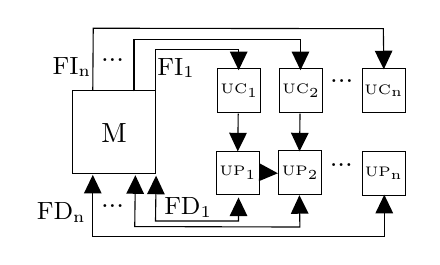
\begin{tikzpicture}[x=0.75pt,y=0.75pt,yscale=-1,xscale=1]
%uncomment if require: \path (0,235); %set diagram left start at 0, and has height of 235

%Shape: Rectangle [id:dp7536045366950691]
\draw   (90.33,80.33) -- (130.33,80.33) -- (130.33,120.33) -- (90.33,120.33) -- cycle ;
%Shape: Rectangle [id:dp09644128938666119]
\draw   (160.33,70) -- (181,70) -- (181,91) -- (160.33,91) -- cycle ;
%Shape: Rectangle [id:dp2241873458228455]
\draw   (159.67,109.67) -- (180.33,109.67) -- (180.33,130.67) -- (159.67,130.67) -- cycle ;
%Straight Lines [id:da17387488972120801]
\draw    (240.49,133.61) -- (240.49,150.61) -- (100.04,150.61) -- (100.04,124.06) ;
\draw [shift={(100.04,121.06)}, rotate = 450] [fill={rgb, 255:red, 0; green, 0; blue, 0 }  ][line width=0.08]  [draw opacity=0] (8.93,-4.29) -- (0,0) -- (8.93,4.29) -- cycle    ;
\draw [shift={(240.49,130.61)}, rotate = 90] [fill={rgb, 255:red, 0; green, 0; blue, 0 }  ][line width=0.08]  [draw opacity=0] (8.93,-4.29) -- (0,0) -- (8.93,4.29) -- cycle    ;
%Straight Lines [id:da8399493952704167]
\draw    (130.52,124.44) -- (130.26,143.28) -- (170.26,143.28) -- (170.26,134.94) ;
\draw [shift={(170.26,131.94)}, rotate = 450] [fill={rgb, 255:red, 0; green, 0; blue, 0 }  ][line width=0.08]  [draw opacity=0] (8.93,-4.29) -- (0,0) -- (8.93,4.29) -- cycle    ;
\draw [shift={(130.56,121.44)}, rotate = 90.77] [fill={rgb, 255:red, 0; green, 0; blue, 0 }  ][line width=0.08]  [draw opacity=0] (8.93,-4.29) -- (0,0) -- (8.93,4.29) -- cycle    ;
%Straight Lines [id:da49329600167598175]
\draw    (170.11,91.5) -- (169.93,106.72) ;
\draw [shift={(169.89,109.72)}, rotate = 270.7] [fill={rgb, 255:red, 0; green, 0; blue, 0 }  ][line width=0.08]  [draw opacity=0] (8.93,-4.29) -- (0,0) -- (8.93,4.29) -- cycle    ;
%Straight Lines [id:da8478353646832082]
\draw    (130.33,80.33) -- (130.33,60.61) -- (170.33,60.61) -- (170.33,67.61) ;
\draw [shift={(170.33,70.61)}, rotate = 270] [fill={rgb, 255:red, 0; green, 0; blue, 0 }  ][line width=0.08]  [draw opacity=0] (8.93,-4.29) -- (0,0) -- (8.93,4.29) -- cycle    ;
%Shape: Rectangle [id:dp901514594846435]
\draw   (190.11,70) -- (210.78,70) -- (210.78,91) -- (190.11,91) -- cycle ;
%Straight Lines [id:da27835153565454673]
\draw    (199.89,91.5) -- (199.7,106.72) ;
\draw [shift={(199.67,109.72)}, rotate = 270.7] [fill={rgb, 255:red, 0; green, 0; blue, 0 }  ][line width=0.08]  [draw opacity=0] (8.93,-4.29) -- (0,0) -- (8.93,4.29) -- cycle    ;
%Straight Lines [id:da807958048653149]
\draw    (119.89,80.83) -- (119.89,55.94) -- (200.11,55.94) -- (200.11,67.61) ;
\draw [shift={(200.11,70.61)}, rotate = 270] [fill={rgb, 255:red, 0; green, 0; blue, 0 }  ][line width=0.08]  [draw opacity=0] (8.93,-4.29) -- (0,0) -- (8.93,4.29) -- cycle    ;
%Shape: Rectangle [id:dp6400885094204286]
\draw   (189.67,109.44) -- (210.33,109.44) -- (210.33,130.44) -- (189.67,130.44) -- cycle ;
%Straight Lines [id:da8803237857270745]
\draw    (180.54,119.83) -- (186.21,120.12) ;
\draw [shift={(189.2,120.27)}, rotate = 182.94] [fill={rgb, 255:red, 0; green, 0; blue, 0 }  ][line width=0.08]  [draw opacity=0] (8.93,-4.29) -- (0,0) -- (8.93,4.29) -- cycle    ;
%Shape: Rectangle [id:dp22681131917528252]
\draw   (229.89,70) -- (250.56,70) -- (250.56,91) -- (229.89,91) -- cycle ;
%Shape: Rectangle [id:dp6689432855617605]
\draw   (229.89,109.78) -- (250.56,109.78) -- (250.56,130.78) -- (229.89,130.78) -- cycle ;
%Straight Lines [id:da6654571954481253]
\draw    (100.04,80.17) -- (100.26,50.39) -- (240.04,50.61) -- (240.23,67.17) ;
\draw [shift={(240.26,70.17)}, rotate = 269.35] [fill={rgb, 255:red, 0; green, 0; blue, 0 }  ][line width=0.08]  [draw opacity=0] (8.93,-4.29) -- (0,0) -- (8.93,4.29) -- cycle    ;
%Straight Lines [id:da8075897242742298]
\draw    (120.52,124.22) -- (120.26,145.94) -- (199.82,146.17) -- (199.64,133.83) ;
\draw [shift={(199.6,130.83)}, rotate = 449.17] [fill={rgb, 255:red, 0; green, 0; blue, 0 }  ][line width=0.08]  [draw opacity=0] (8.93,-4.29) -- (0,0) -- (8.93,4.29) -- cycle    ;
\draw [shift={(120.56,121.22)}, rotate = 90.68] [fill={rgb, 255:red, 0; green, 0; blue, 0 }  ][line width=0.08]  [draw opacity=0] (8.93,-4.29) -- (0,0) -- (8.93,4.29) -- cycle    ;

% Text Node
\draw (110.33,100.67) node   [align=left] {M};
% Text Node
\draw (170.67,80.5) node   [align=left] {{\tiny UC\textsubscript{1}}};
% Text Node
\draw (170,120.17) node   [align=left] {{\tiny UP\textsubscript{1}}};
% Text Node
\draw (146,136.67) node   [align=left] {{\small FD\textsubscript{1}}};
% Text Node
\draw (140.22,69.56) node   [align=left] {{\small FI\textsubscript{1}}};
% Text Node
\draw (200.44,80.5) node   [align=left] {{\tiny UC\textsubscript{2}}};
% Text Node
\draw (220,75.67) node   [align=left] {...};
% Text Node
\draw (109.56,65.67) node   [align=left] {...};
% Text Node
\draw (200,119.94) node   [align=left] {{\tiny UP\textsubscript{2}}};
% Text Node
\draw (240.22,80.5) node   [align=left] {{\tiny UC\textsubscript{n}}};
% Text Node
\draw (240.22,120.28) node   [align=left] {{\tiny UP\textsubscript{n}}};
% Text Node
\draw (84.89,139.11) node   [align=left] {{\small FD\textsubscript{n}}};
% Text Node
\draw (90,69.11) node   [align=left] {{\small FI\textsubscript{n}}};
% Text Node
\draw (219.78,116.11) node   [align=left] {...};
% Text Node
\draw (109.56,135.89) node   [align=left] {...};
\end{tikzpicture}
                           \\
\end{tabular}
\end{center}
\caption{Clasificación de Flynn de arquitecturas}
\end{figure}

\pagebreak

\textbf{Arquitecturas SISD}

Corresponden a computadores uni-procesador, en los que se evalúa una instrucción y un dato cada vez.
Siguen una estructura puramente secuencial y no permiten paralelismo.

\begin{lstlisting}[language=Pascal]
for i in 1 to 4 do
	C[i] = A[i] + B[i]
	F[i] = D[i] - E[i]
	K[i] = H[i] * G[i]
done
\end{lstlisting}

\textbf{Arquitecturas SIMD}

Aprovechan el paralelismo de datos para poder procesar un número de datos mayor en cada operación.
Es el caso de los operadores vectoriales, que permiten trabajar con vectores mediantes instrucciones como \code{ADDV}, \code{SUBV} o \code{MULV}.
Estas instrucciones permiten trabajar directamente con elementos de vectores con mayor rendimiento.
Por su parte, los procesadores matriciales permiten trabajar con vectorialmente con múltiples vectores (por ejemplo, con matrices $EP_i$).

\begin{lstlisting}[language=Pascal]
for all EPi(i in 1 to 4) do
	C[i] = A[i] + B[i]
	F[i] = D[i] - E[i]
	K[i] = H[i] * G[i]
done
\end{lstlisting}

En este caso, el procesador vectorial ejecutará el bucle \code{for all} cuatro veces, aprovechando en cada una el paralelismo de las instrucciones \code{ADDV}, \code{SUBV} y \code{MULV}.

\textbf{Arquitecturas MISD}

Aunque podemos simular este modelo en un código para programas que procesan secuencias o flujos de datos, no sexisten computadores que funcionen con esta arquitectura.

\textbf{Arquitecturas MIMD}

Es la arquitectura de las máquinas multinúcleo, multiprocesador y multicomputador.
Esta multitud de componentes hace que puedan aprovechar el paralelismo a nivel de procesos.

\pagebreak

\begin{lstlisting}[language=Pascal]
{Proceso 1}
for i in 1 to 4 do
	C[i] = A[i] + B[i]
done
{Proceso 2}
for i in 1 to 4 do
	F[i] = D[i] - E[i]
done
{Proceso 3}
for i in 1 to 4 do
	K[i] = H[i] * G[i]
done
\end{lstlisting}

\subsubsection{Clasificación según el sistema de memoria}

\textbf{Multiprocesadores}

\begin{figure}[h]
\begin{center}
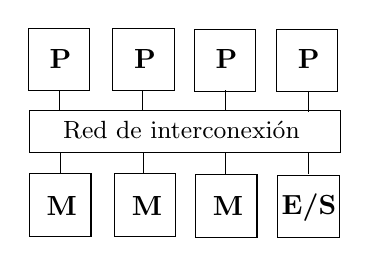
\begin{tikzpicture}[x=0.75pt,y=0.75pt,yscale=-1,xscale=1]
%uncomment if require: \path (0,235); %set diagram left start at 0, and has height of 235

%Shape: Rectangle [id:dp1388771205713386]
\draw   (90.6,79.74) -- (240.38,79.74) -- (240.38,99.82) -- (90.6,99.82) -- cycle ;
%Shape: Rectangle [id:dp7715938821633621]
\draw   (90,39.98) -- (119.59,39.98) -- (119.59,70) -- (90,70) -- cycle ;
%Shape: Rectangle [id:dp2149759037343656]
\draw   (130.8,39.98) -- (160.39,39.98) -- (160.39,70) -- (130.8,70) -- cycle ;
%Shape: Rectangle [id:dp48718644358649077]
\draw   (170,40.38) -- (199.59,40.38) -- (199.59,70.4) -- (170,70.4) -- cycle ;
%Shape: Rectangle [id:dp4526044131265844]
\draw   (209.6,40.58) -- (239.19,40.58) -- (239.19,70.6) -- (209.6,70.6) -- cycle ;
%Shape: Rectangle [id:dp974079393192987]
\draw   (90.65,110.18) -- (120.24,110.18) -- (120.24,140.2) -- (90.65,140.2) -- cycle ;
%Shape: Rectangle [id:dp6514697889359573]
\draw   (131.45,110.18) -- (161.04,110.18) -- (161.04,140.2) -- (131.45,140.2) -- cycle ;
%Shape: Rectangle [id:dp3675260839451622]
\draw   (170.65,110.58) -- (200.24,110.58) -- (200.24,140.6) -- (170.65,140.6) -- cycle ;
%Shape: Rectangle [id:dp5150776265573659]
\draw   (210.25,110.78) -- (239.84,110.78) -- (239.84,140.8) -- (210.25,140.8) -- cycle ;
%Straight Lines [id:da8737015330323414]
\draw    (104.98,69.77) -- (104.98,79.8) ;
%Straight Lines [id:da2156293649560963]
\draw    (144.98,69.97) -- (144.98,80) ;
%Straight Lines [id:da6056566302075724]
\draw    (104.98,69.77) -- (104.98,79.8) ;
%Straight Lines [id:da001765354038316902]
\draw    (144.98,69.97) -- (144.98,80) ;
%Straight Lines [id:da2798932998598058]
\draw    (185.18,69.97) -- (185.18,80) ;
%Straight Lines [id:da6563141101138771]
\draw    (225.18,70.17) -- (225.18,80.2) ;
%Straight Lines [id:da5650083821579299]
\draw    (105.43,99.77) -- (105.43,109.8) ;
%Straight Lines [id:da2651094160788827]
\draw    (145.43,99.97) -- (145.43,110) ;
%Straight Lines [id:da025547387273394784]
\draw    (185.18,99.97) -- (185.18,110) ;
%Straight Lines [id:da95584766517231]
\draw    (225.18,100.17) -- (225.18,110.2) ;

% Text Node
\draw (105.6,83.74) node [anchor=north west][inner sep=0.75pt]   [align=left] {\small Red de interconexión};
% Text Node
\draw (99,49) node [anchor=north west][inner sep=0.75pt]   [align=left] {\textbf{P}};
% Text Node
\draw (139.8,49) node [anchor=north west][inner sep=0.75pt]   [align=left] {\textbf{P}};
% Text Node
\draw (179,49) node [anchor=north west][inner sep=0.75pt]   [align=left] {\textbf{P}};
% Text Node
\draw (218.6,49) node [anchor=north west][inner sep=0.75pt]   [align=left] {\textbf{P}};
% Text Node
\draw (97.65,120) node [anchor=north west][inner sep=0.75pt]   [align=left] {\textbf{M}};
% Text Node
\draw (138.65,120) node [anchor=north west][inner sep=0.75pt]   [align=left] {\textbf{M}};
% Text Node
\draw (177.65,120) node [anchor=north west][inner sep=0.75pt]   [align=left] {\textbf{M}};
% Text Node
\draw (210.85,118.5) node [anchor=north west][inner sep=0.75pt]   [align=left] {\textbf{E/S}};
\end{tikzpicture}

\end{center}
\caption{Arquitectura multiprocesador con memoria centralizada (SMP)}
\end{figure}

Son aquellos en los que todos los procesadores comparten el mismo espacio de direcciones, permitiendo al programador trabajar sin necesitar conocer dónde están almacenados los datos.
La comunicación entre procesos se hace explícita mediante variables compartidas, de forma que no existe varias instancias del mismo dato en memoria principal.
Sin enbargo, la latencia de las operaciones es alta y el sistema es poco escalable, ya que requiere aumentar la caché dle procesador, usar redes de menor latencia y ancho de banda que un bus y distribuir físicamente los módulos de memoria entre los procesadores sin dejar de compartir el espacio de direcciones.

Debido a que la distribución de código y datos entre procesadores no es necesaria en estas arquitecturas y que la sincronización se implementa mediante primitivas, programar en arquitecturas SMP es, generalmente, más sencillo que en arquitecturas multicomputador.

\textbf{Multicomputadores}

\begin{figure}[h]
\begin{center}
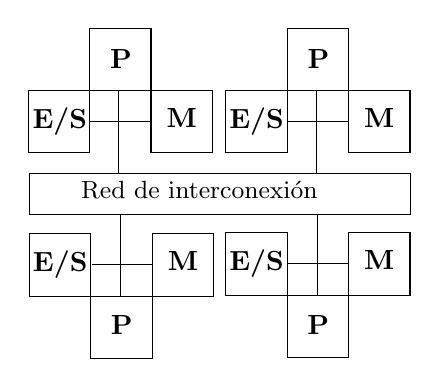
\begin{tikzpicture}[x=0.75pt,y=0.75pt,yscale=-1,xscale=1]
%uncomment if require: \path (0,235); %set diagram left start at 0, and has height of 235

%Shape: Rectangle [id:dp1388771205713386]
\draw   (90.6,79.74) -- (274.09,79.74) -- (274.09,99.82) -- (90.6,99.82) -- cycle ;
%Shape: Rectangle [id:dp7715938821633621]
\draw   (90,39.98) -- (119.59,39.98) -- (119.59,70) -- (90,70) -- cycle ;
%Shape: Rectangle [id:dp2149759037343656]
\draw   (119.59,9.96) -- (149.17,9.96) -- (149.17,39.98) -- (119.59,39.98) -- cycle ;
%Shape: Rectangle [id:dp48718644358649077]
\draw   (149.17,39.98) -- (178.76,39.98) -- (178.76,70) -- (149.17,70) -- cycle ;
%Straight Lines [id:da8737015330323414]
\draw    (119.89,54.78) -- (149.29,54.78) ;
%Straight Lines [id:da6056566302075724]
\draw    (133.58,40.18) -- (133.58,79.6) ;
%Shape: Rectangle [id:dp7215848085922171]
\draw   (185.2,39.98) -- (214.79,39.98) -- (214.79,70) -- (185.2,70) -- cycle ;
%Shape: Rectangle [id:dp38227489239846646]
\draw   (214.79,9.96) -- (244.37,9.96) -- (244.37,39.98) -- (214.79,39.98) -- cycle ;
%Shape: Rectangle [id:dp8117581367578898]
\draw   (244.37,39.98) -- (273.96,39.98) -- (273.96,70) -- (244.37,70) -- cycle ;
%Straight Lines [id:da5970149414950394]
\draw    (215.09,54.78) -- (244.49,54.78) ;
%Straight Lines [id:da5490790011884338]
\draw    (228.78,40.18) -- (228.78,79.6) ;
%Shape: Rectangle [id:dp2328821300848748]
\draw   (90.6,108.98) -- (120.19,108.98) -- (120.19,139) -- (90.6,139) -- cycle ;
%Shape: Rectangle [id:dp6525667710060407]
\draw   (120.19,139) -- (149.77,139) -- (149.77,169.02) -- (120.19,169.02) -- cycle ;
%Shape: Rectangle [id:dp25124533437909113]
\draw   (149.77,108.98) -- (179.36,108.98) -- (179.36,139) -- (149.77,139) -- cycle ;
%Straight Lines [id:da27708443377640635]
\draw    (120.49,123.78) -- (149.89,123.78) ;
%Straight Lines [id:da4001865768217636]
\draw    (134.58,99.98) -- (134.58,139.4) ;
%Shape: Rectangle [id:dp6873478861133927]
\draw   (185.2,108.58) -- (214.79,108.58) -- (214.79,138.6) -- (185.2,138.6) -- cycle ;
%Shape: Rectangle [id:dp009912235254289747]
\draw   (214.79,138.6) -- (244.37,138.6) -- (244.37,168.62) -- (214.79,168.62) -- cycle ;
%Shape: Rectangle [id:dp309969046128054]
\draw   (244.37,108.58) -- (273.96,108.58) -- (273.96,138.6) -- (244.37,138.6) -- cycle ;
%Straight Lines [id:da9264242146449485]
\draw    (215.09,123.38) -- (244.49,123.38) ;
%Straight Lines [id:da9097877564188441]
\draw    (229.18,99.58) -- (229.18,139) ;

% Text Node
\draw (114.2,82.54) node [anchor=north west][inner sep=0.75pt]   [align=left] {\small Red de interconexión};
% Text Node
\draw (90.8,47) node [anchor=north west][inner sep=0.75pt]   [align=left] {\textbf{E/S}};
% Text Node
\draw (128.2,19) node [anchor=north west][inner sep=0.75pt]   [align=left] {\textbf{P}};
% Text Node
\draw (155.4,47.4) node [anchor=north west][inner sep=0.75pt]   [align=left] {\textbf{M}};
% Text Node
\draw (185.6,47) node [anchor=north west][inner sep=0.75pt]   [align=left] {\textbf{E/S}};
% Text Node
\draw (223.4,19) node [anchor=north west][inner sep=0.75pt]   [align=left] {\textbf{P}};
% Text Node
\draw (250.6,47.4) node [anchor=north west][inner sep=0.75pt]   [align=left] {\textbf{M}};
% Text Node
\draw (91,116) node [anchor=north west][inner sep=0.75pt]   [align=left] {\textbf{E/S}};
% Text Node
\draw (128.6,147) node [anchor=north west][inner sep=0.75pt]   [align=left] {\textbf{P}};
% Text Node
\draw (156,116.4) node [anchor=north west][inner sep=0.75pt]   [align=left] {\textbf{M}};
% Text Node
\draw (185.6,115.6) node [anchor=north west][inner sep=0.75pt]   [align=left] {\textbf{E/S}};
% Text Node
\draw (223.2,147) node [anchor=north west][inner sep=0.75pt]   [align=left] {\textbf{P}};
% Text Node
\draw (250.6,116) node [anchor=north west][inner sep=0.75pt]   [align=left] {\textbf{M}};
\end{tikzpicture}

\end{center}
\caption{Arquitectura multicomputador}
\end{figure}

Son aquellos en los que cada procesador tiene un espacio de direcciones propio, por lo que el programador debe conocer dónde están almacenados los datos con los que opera.
La comunicación entre procesos se hace explícita mediante programas de paso de mensajes, de forma que eisten múltiples instancias de los datos en memoria principal, ya que tienen que leerse por la memoria de cada computador individual.
Como contrapartida a esta complejidad, la latencia de las operaciones es baja y el sistema es más escalable, ya que únicamente requiere conectar más computadores al sistema de paso de mensajes.

Debido a que la distribución de código y datos entre los procesadores es necesaria, lo que conlleva a usar herramientas de programación más sofisticadas, y que la sincronización entre procesos se hace mediante programas de comunicación, la programación en arquitecturas multicomputador es, generalmente, más difícil que en arquitecturas SMP\@.

\textbf{Comunicación \textit{uno a uno} en SMP y multicomputador}

En las arquitecturas SMP, la comunicación \textit{uno a uno}, que se abordará en~\ref{herramientas-codigo-par}, se da mediante accesos concurrentes a la memoria principal, de forma que un nodo fuente esnvía una dirección a un nodo destino y esperan a una respuesta del otro para poder seguir operando.
Esta sincronización se conoce como el \textbf{problema del productor-consumidor}\footnote{Sistemas concurrentes y distribuidos, tema 1}.

En las arquitecturas multicomputador, la red de comunicación es un búfer de datos gestionado por un programa de paso de mensajes que recibe peticiones de envío y recepción de datos y las coordina adecuadamente para garantizar que se cumplen las propiedades de seguridad y vivacidad del sistema.
Debido a la estructura de esta red de comunicación, las funciones de recepción de mensajes son bloqueantes para el proceso receptor.

\textbf{Incremento de escalabilidad en multiprocesadores}

Las arquitecturas multiprocesador presentan un gran inconveniente en su escalabilidad con respecto a las arquitecturas multicomputador.
Mientras las últimas requieren poco más que instalar un nuevo sistema en la red de comunicación, las primeras requieren que se realicen modificaciones estructurales sobre el sistema, como aumentar la cache de los procesadores, usar redes de menor latencia y ancho de banda que un bus y distribuir físicamente los módulos de memoria entre los procesadores asegurando que se siga compartiendo el espacio de direcciones.

\subsubsection{Clasificación según el sistema de memoria}

Debido a que las arquitecturas multicomputador están compuestas por diferentes máquinas con sus módulos de procesamiento, E/S y memoria independientes, éstas siguen el sistema de memoria \textbf{NORMA} (\textit{No Remote Memory Access}).

Por otro lado, las arquitecturas multiprocesador sí comparten memoria en un único espacio de direcciones.
Esta memoria puede ser uniforme (\textbf{NUMA}) o no (\textbf{UMA}).

\textbf{NUMA (\textit{Non-Uniform Memory Access})}

Este tipo de memoria, que también puede ser utilizada en redes multicomputador, se caracteriza porque el tiempo de acceso depende de la ubicación de la memoria relativa al procesador que realiza la petición de acceso, siendo el acceso a la memoria local al procesador más rápido que a las memorias externas.
Una variante de esta memoria es \textbf{CC-NUMA} (\textit{Cache Coherent NUMA}).
Aunque mantener coherencia en la caché en memorias NUMA lleva consigo una gran sobrecarga (\ref{ganancia-prestaciones-escalabilidad}), la escalabilidad de las memorias NUMA sin coherencia en caché son prohibitivamente complejas de gestionar, por lo que se prefiere utilizar memorias CC-NUMA por mucho que ofrezcan un muy bajo rendimiento cuando varios procesadores intentan acceder en sucesiones rápidas a la misma dirección de memoria.

Como caso particular de las memorias NUMA, las memorias \textbf{COMA} (\textit{Cache-Only Memory Architecture}) sólo trabajan con cachés, de forma que un acceso a un dato en memoria puede hacer que éste migre a otra.
Esto reduce el número de copias redundantes de los datos a lo largo del sistema, pero plantea problemas de ubicación de los datos y las acciones a realizar al llenarse el sistema mememoria, que suelen subsanarse mediante mecanismos de hardware de coherencia de memoria.

\textbf{UMA (\textit{Uniform Memory Access})}

En este sistema, todos los procesadores comparten uniformemente la misma memoria física, de forma que los accesos a la misma son de igual para todos los procesadores y no existe redundancia de datos en la memoria principal (aunque podría existirla en la caché de los procesadores).
Es el tipo de memoria utilizada por las arquitecturas SMP\@.
